% ৪.৩ World Wide Web, Web Browser ও Search Engine
\section{World Wide Web, Web Browser ও Search Engine}

\begin{learningbox}
এই টপিক শেষে শিক্ষার্থী পারবে:
\begin{itemize}
\item World Wide Web বা WWW-এর সংজ্ঞা, উৎপত্তি ও কাজ ব্যাখ্যা করতে।
\item Internet ও WWW-এর পার্থক্য লিখতে।
\item Web browser-এর কাজ ও উদাহরণ বলতে।
\item Search engine-এর কাজ, ধাপ ও ব্যবহার ব্যাখ্যা করতে।
\item Browser ও search engine-এর পার্থক্য বুঝতে।
\end{itemize}
\end{learningbox}

\subsection{ভূমিকা}

ওয়েব ডিজাইন বুঝতে হলে তিনটি বিষয় ভালোভাবে জানা দরকার - World Wide Web বা WWW, Web Browser এবং Search Engine। কারণ HTML দিয়ে ওয়েবপেজ তৈরি করা হলেও user সেই ওয়েবপেজ দেখে web browser-এর মাধ্যমে। আবার নির্দিষ্ট website বা প্রয়োজনীয় তথ্য খুঁজে পাওয়ার জন্য search engine ব্যবহার করা হয়।

সংক্ষেপে বলা যায়, WWW হলো web resource-এর বিশাল ব্যবস্থা, browser হলো সেই resource দেখার software এবং search engine হলো WWW থেকে প্রয়োজনীয় তথ্য খুঁজে বের করার tool।

\begin{center}
\scaletikz{\begin{tikzpicture}[
  browser/.style={draw, rounded corners, fill=gray!4, minimum width=10.5cm, minimum height=5.55cm},
  bar/.style={draw, rounded corners, fill=white, minimum height=0.45cm, align=left, font=\scriptsize},
  content/.style={draw, rounded corners, fill=blue!4, align=center, font=\scriptsize},
  label/.style={draw, rounded corners, fill=yellow!15, align=center, font=\scriptsize, inner xsep=3pt, inner ysep=2pt},
  arrow/.style={bookarrow}
]
\node[browser] (win) {};
\node[font=\small\bfseries] at ([yshift=2.55cm]win.center) {Web Browser Window};
\node[bar, minimum width=7.35cm] (urlbar) at ([xshift=-0.8cm,yshift=2.05cm]win.center) {\texttt{https://www.abccollege.edu.bd}};
\node[bar, minimum width=1.35cm] (reload) at ([xshift=4.35cm,yshift=2.05cm]win.center) {Go};
\node[content, minimum width=2.1cm, minimum height=0.52cm] (logo) at ([xshift=-3.0cm,yshift=1.25cm]win.center) {ABC College};
\node[content, minimum width=4.85cm, minimum height=0.52cm] (nav) at ([xshift=1.15cm,yshift=1.25cm]win.center) {Home \quad Notice \quad Result \quad Contact};
\node[content, minimum width=8.3cm, minimum height=1.0cm] (hero) at ([yshift=0.3cm]win.center) {Homepage content\\welcome text, image/banner, important notice};
\node[content, minimum width=3.95cm, minimum height=0.7cm] (link) at ([xshift=-2.25cm,yshift=-1.0cm]win.center) {Hyperlink: Result};
\node[content, minimum width=3.95cm, minimum height=0.7cm] (page) at ([xshift=2.25cm,yshift=-1.0cm]win.center) {Webpage area};
\node[bar, minimum width=5.85cm] (search) at ([yshift=-2.0cm]win.center) {Search box: \texttt{HSC ICT result}};

\node[label, anchor=east] (lbrowser) at ([xshift=-5.45cm,yshift=2.55cm]win.center) {Browser};
\node[label, anchor=east] (lurl) at ([xshift=-5.2cm,yshift=1.55cm]win.center) {URL bar};
\node[label, anchor=west] (lwebsite) at ([xshift=5.2cm,yshift=1.25cm]win.center) {Website name};
\node[label, anchor=west] (lnav) at ([xshift=5.15cm,yshift=0.45cm]win.center) {Navigation};
\node[label, anchor=east] (lhome) at ([xshift=-5.2cm,yshift=0.15cm]win.center) {Homepage};
\node[label, anchor=east] (lsearch) at ([xshift=-5.2cm,yshift=-2.25cm]win.center) {Search bar};
\node[label, anchor=east] (llink) at ([xshift=-5.3cm,yshift=-1.1cm]win.center) {Link};

\draw[bookarrow] (lbrowser.east) -- (win.north west);
\draw[bookarrow] (lurl.east) -- (urlbar.west);
\draw[bookarrow] (lwebsite.west) -- (logo.east);
\draw[bookarrow] (lnav.west) -- (nav.east);
\draw[bookarrow] (lhome.east) -- (hero.west);
\draw[bookarrow] (lsearch.east) -- (search.west);
\draw[bookarrow] (llink.east) -- (link.west);
\end{tikzpicture}}\\[3pt]
\textit{চিত্র: Browser window-এ URL bar, website, homepage, navigation, hyperlink ও search bar}
\end{center}

\begin{center}
\scaletikz{\begin{tikzpicture}[
  box/.style={draw, rounded corners, fill=green!6, minimum width=2.55cm, minimum height=0.78cm, align=center, font=\small},
  wide/.style={draw, rounded corners, fill=blue!6, minimum width=3.2cm, minimum height=0.78cm, align=center, font=\small},
  arrow/.style={bookarrow}
]
\node[wide] (www) {WWW\\Web resources};
\node[box, below left=0.95cm and 1.65cm of www] (browser) {Web Browser};
\node[box, below right=0.95cm and 1.65cm of www] (search) {Search Engine};
\node[wide, below=1.1cm of www] (site) {Website / Webpage};
\draw[bookarrow] (browser) -- node[left, font=\scriptsize]{opens} (site);
\draw[bookarrow] (search) -- node[right, font=\scriptsize]{finds} (site);
\draw[bookarrow] (site) -- node[left, font=\scriptsize]{part of} (www);
\draw[bookarrow] (browser) -- node[above, font=\scriptsize]{uses URL} (www);
\draw[bookarrow] (search) -- node[above, font=\scriptsize]{indexes} (www);
\end{tikzpicture}}\\[3pt]
\textit{চিত্র: WWW, browser ও search engine-এর সম্পর্ক}
\end{center}

\subsection{World Wide Web বা WWW}

\subsubsection{WWW কী?}

\begin{definitionbox}{World Wide Web}
ইন্টারনেটের মাধ্যমে পরস্পর সংযুক্ত hypertext document, webpage, image, video ও অন্যান্য web resource প্রদর্শন ও ব্যবহারের ব্যবস্থাকে World Wide Web বা WWW বলে।
\end{definitionbox}

World Wide Web-কে সংক্ষেপে Web বলা হয়। Web-এর মাধ্যমে user hyperlink ব্যবহার করে এক webpage থেকে অন্য webpage-এ যেতে পারে। Website, webpage, hyperlink, URL, browser এবং web server - এগুলো WWW ব্যবস্থার গুরুত্বপূর্ণ অংশ।

\begin{boardbox}{পরীক্ষার সংক্ষিপ্ত উত্তর}
World Wide Web বা WWW হলো internet-এর মাধ্যমে পরস্পর সংযুক্ত hypertext document ও web resource ব্যবহারের একটি ব্যবস্থা। ব্যবহারকারী web browser-এর মাধ্যমে WWW থেকে website ও webpage দেখতে পারে।
\end{boardbox}

\subsubsection{WWW-এর উৎপত্তি}

WWW-এর ধারণা দেন ব্রিটিশ computer scientist Tim Berners-Lee। তিনি ১৯৮৯ সালে CERN-এ কাজ করার সময় World Wide Web-এর ধারণা উপস্থাপন করেন। এর মূল উদ্দেশ্য ছিল গবেষক ও বিজ্ঞানীদের মধ্যে সহজে তথ্য বিনিময়ের ব্যবস্থা তৈরি করা।

\begin{boardbox}{Big Scientist Contribution}
\begin{center}
\begin{tabular}{|p{0.25\textwidth}|p{0.18\textwidth}|p{0.43\textwidth}|}
\hline
\textbf{নাম/প্রতিষ্ঠান} & \textbf{সাল} & \textbf{অবদান} \\
\hline
Tim Berners-Lee & 1989--1991 & WWW-এর ধারণা দেন; HTML, HTTP, URL ধারণা এবং প্রথম web browser/server তৈরিতে প্রধান ভূমিকা রাখেন \\
\hline
Robert Cailliau & 1990 & Web project-এর formal proposal তৈরিতে Tim Berners-Lee-এর সাথে কাজ করেন \\
\hline
CERN & 1989--1991 & WWW-এর জন্মস্থান; গবেষকদের তথ্য বিনিময়ের প্রয়োজন থেকে Web project শুরু হয় \\
\hline
W3C & 1994 & Web standard উন্নয়ন, HTML/CSS/accessibility guideline রক্ষণাবেক্ষণে কাজ করে \\
\hline
WHATWG & 2004 থেকে & আধুনিক HTML Living Standard উন্নয়নে গুরুত্বপূর্ণ ভূমিকা রাখে \\
\hline
\end{tabular}
\end{center}
\end{boardbox}

\begin{examplebox}{Web Timeline}
\begin{center}
\begin{tabular}{|p{0.18\textwidth}|p{0.66\textwidth}|}
\hline
\textbf{সাল} & \textbf{ঘটনা} \\
\hline
1989 & Tim Berners-Lee CERN-এ World Wide Web-এর প্রস্তাব দেন \\
\hline
1990 & Tim Berners-Lee ও Robert Cailliau Web proposal formal করেন \\
\hline
1990 & প্রথম web server ও browser/editor তৈরির কাজ শুরু হয় \\
\hline
1991 & Web publicভাবে পরিচিত হতে শুরু করে; প্রথমদিকের webpage HTML দিয়ে তৈরি হয় \\
\hline
1994 & W3C প্রতিষ্ঠিত হয় web standard উন্নয়নের জন্য \\
\hline
বর্তমান & WWW বিশ্বব্যাপী website, webpage, web application ও online service-এর ভিত্তি \\
\hline
\end{tabular}
\end{center}
\end{examplebox}

\begin{keypointbox}{Exam note}
\begin{itemize}
\item WWW-এর পূর্ণরূপ: World Wide Web।
\item WWW-এর উদ্ভাবক: Tim Berners-Lee।
\item উদ্ভাবনের সাল: 1989।
\item প্রতিষ্ঠান: CERN।
\item WWW internet-এর একটি গুরুত্বপূর্ণ service।
\end{itemize}
\end{keypointbox}

\subsubsection{WWW কীভাবে কাজ করে?}

WWW client-server পদ্ধতিতে কাজ করে। User browser-এ কোনো website address বা URL লিখলে browser web server-এ request পাঠায়। Server সেই request অনুযায়ী HTML, CSS, image, JavaScript ইত্যাদি file browser-এ পাঠায়। এরপর browser সেগুলো process করে user-এর সামনে webpage আকারে দেখায়।

\begin{center}
\begin{tikzpicture}[
  box/.style={draw, rounded corners, fill=green!6, minimum width=2.45cm, minimum height=0.78cm, align=center, font=\small},
  data/.style={draw, rounded corners, fill=blue!6, minimum width=2.8cm, minimum height=0.78cm, align=center, font=\small},
  arrow/.style={->, thick}
]
\node[box] (user) {User};
\node[box, right=0.65cm of user] (browser) {Browser};
\node[box, right=0.65cm of browser] (server) {Web Server};
\node[data, below=0.85cm of server] (res) {HTML/CSS/Image\\Response};
\node[box, below=0.85cm of browser] (out) {Browser\\Output};
\draw[arrow] (user) -- (browser);
\draw[arrow] (browser) -- node[above, font=\scriptsize]{request} (server);
\draw[arrow] (server) -- (res);
\draw[arrow] (res) -- node[below, font=\scriptsize]{render} (out);
\draw[arrow] (out) -- (user);
\end{tikzpicture}\\[3pt]
\textit{চিত্র: WWW client-server পদ্ধতিতে কাজ করে}
\end{center}

\subsubsection{WWW-এর বৈশিষ্ট্য}

\begin{itemize}
\item WWW internet-এর উপর ভিত্তি করে কাজ করে।
\item এতে webpage ও website hyperlink-এর মাধ্যমে যুক্ত থাকে।
\item browser দিয়ে WWW access করা যায়।
\item URL ব্যবহার করে web resource খুঁজে পাওয়া যায়।
\item HTTP/HTTPS protocol ব্যবহার করে তথ্য আদান-প্রদান হয়।
\item text, image, audio, video, animation ও document প্রদর্শন করা যায়।
\item এটি বিশ্বব্যাপী তথ্য প্রকাশ ও ব্যবহারের সহজ মাধ্যম।
\end{itemize}

\subsection{WWW ও Internet-এর পার্থক্য}

অনেক শিক্ষার্থী WWW ও Internet-কে একই মনে করে। কিন্তু এরা একই জিনিস নয়। Internet হলো বিশ্বব্যাপী computer network, আর WWW হলো সেই internet ব্যবহার করে webpage ও web resource access করার ব্যবস্থা।

\begin{center}
\begin{tabular}{|p{0.20\textwidth}|p{0.32\textwidth}|p{0.32\textwidth}|}
\hline
\textbf{বিষয়} & \textbf{Internet} & \textbf{WWW} \\
\hline
অর্থ & বিশ্বব্যাপী সংযুক্ত computer network & Internet ব্যবহার করে webpage/resource দেখার ব্যবস্থা \\
\hline
প্রকৃতি & Hardware, cable, router, server ও network infrastructure & Hypertext document ও web resource system \\
\hline
ব্যবহার & Email, file transfer, VoIP, web browsing ইত্যাদি & Website ও webpage দেখা \\
\hline
সম্পর্ক & WWW চালাতে Internet দরকার & Internet-এর একটি service \\
\hline
উদাহরণ & ISP, router, cable, server network & website, webpage, hyperlink \\
\hline
\end{tabular}
\end{center}

\begin{examplebox}{সহজ উদাহরণ}
Internet হলো রাস্তা বা যোগাযোগের অবকাঠামো, আর WWW হলো সেই রাস্তা ব্যবহার করে চলা web service। তাই Internet না থাকলে WWW ব্যবহার করা যায় না, কিন্তু Internet শুধু WWW নয়; email, file transfer, online game, video call ইত্যাদিও Internet ব্যবহার করে।
\end{examplebox}

\subsection{Web Browser}

\subsubsection{Web Browser কী?}

\begin{definitionbox}{Web Browser}
WWW থেকে তথ্য অনুসন্ধান, আহরণ, প্রদর্শন ও সংরক্ষণের জন্য ব্যবহৃত application software-কে web browser বলে।
\end{definitionbox}

Web browser user-এর device-এ install করা থাকে। Browser website-এর HTML, CSS, image, video ইত্যাদি গ্রহণ করে user-এর সামনে readable webpage হিসেবে প্রদর্শন করে।

\begin{examplebox}{উদাহরণ}
Google Chrome, Mozilla Firefox, Microsoft Edge, Safari, Opera ইত্যাদি web browser-এর উদাহরণ।
\end{examplebox}

\subsubsection{Web Browser-এর কাজ}

\begin{keypointbox}{Browser-এর প্রধান কাজ}
\begin{itemize}
\item ওয়েবপেজ প্রদর্শন করা।
\item URL অনুযায়ী server-এ request পাঠানো।
\item HTML, CSS ও JavaScript interpret করে output দেখানো।
\item image, audio, video ও document প্রদর্শন করা।
\item hyperlink follow করা।
\item file download করতে সাহায্য করা।
\item bookmark, history ও save সুবিধা দেওয়া।
\item webpage print করা।
\item form submit ও login page ব্যবহার করতে সাহায্য করা।
\end{itemize}
\end{keypointbox}

\subsubsection{Browser কীভাবে webpage দেখায়?}

একটি webpage browser-এ দেখানোর সাধারণ ধাপ হলো:

\begin{enumerate}
\item User browser-এ URL লেখে।
\item Browser DNS-এর সাহায্যে domain-এর IP address খুঁজে পায়।
\item Browser web server-এ request পাঠায়।
\item Server HTML, CSS, image ও অন্যান্য file পাঠায়।
\item Browser HTML code পড়ে webpage তৈরি করে।
\item User browser window-তে webpage দেখে।
\end{enumerate}

\begin{boardbox}{মনে রাখো}
Browser নিজে website তৈরি করে না; browser website-এর file server থেকে এনে user-এর সামনে প্রদর্শন করে।
\end{boardbox}

\subsection{Browser ও Search Engine-এর পার্থক্য}

\begin{center}
\begin{tabular}{|p{0.20\textwidth}|p{0.32\textwidth}|p{0.32\textwidth}|}
\hline
\textbf{বিষয়} & \textbf{Web Browser} & \textbf{Search Engine} \\
\hline
অর্থ & webpage দেখার application software & তথ্য খোঁজার online tool/service \\
\hline
কাজ & website খুলে দেখায় & keyword অনুযায়ী website বা তথ্য খুঁজে দেয় \\
\hline
ব্যবহার & URL লিখে website visit করা & keyword লিখে result পাওয়া \\
\hline
উদাহরণ & Chrome, Firefox, Edge, Safari & Google, Bing, Yahoo, DuckDuckGo \\
\hline
সম্পর্ক & search engine access করতে browser লাগে & browser-এর মাধ্যমে search engine ব্যবহার করা হয় \\
\hline
\end{tabular}
\end{center}

\begin{examplebox}{সহজ উদাহরণ}
Chrome হলো browser, আর Google Search হলো search engine। Google ব্যবহার করতে Chrome, Firefox বা অন্য কোনো browser লাগে।
\end{examplebox}

\subsection{Search Engine}

\subsubsection{Search Engine কী?}

\begin{definitionbox}{Search Engine}
ইন্টারনেট থেকে প্রয়োজনীয় তথ্য, webpage, image, video বা document খুঁজে পাওয়ার জন্য ব্যবহৃত web-based tool বা software system-কে search engine বলে।
\end{definitionbox}

Search engine user-এর দেওয়া keyword অনুযায়ী internet থেকে relevant website বা webpage খুঁজে result হিসেবে দেখায়।

\begin{examplebox}{উদাহরণ}
Google, Bing, Yahoo, DuckDuckGo, Baidu ইত্যাদি search engine-এর উদাহরণ।
\end{examplebox}

\begin{center}
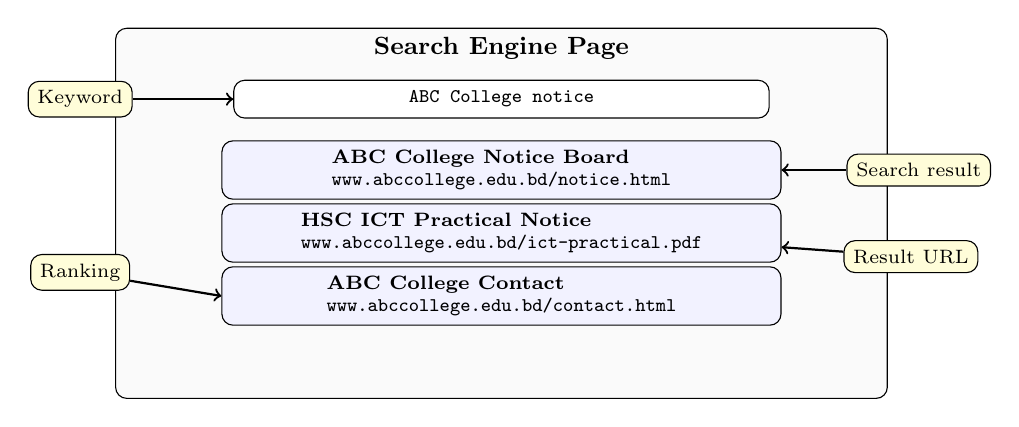
\begin{tikzpicture}[
  page/.style={draw, rounded corners, fill=gray!4, minimum width=9.8cm, minimum height=4.7cm},
  bar/.style={draw, rounded corners, fill=white, minimum height=0.48cm, align=left, font=\scriptsize},
  result/.style={draw, rounded corners, fill=blue!5, minimum width=7.1cm, minimum height=0.55cm, align=left, font=\scriptsize},
  label/.style={draw, rounded corners, fill=yellow!15, align=center, font=\scriptsize},
  arrow/.style={->, thick}
]
\node[page] (searchpage) {};
\node[font=\small\bfseries] at ([yshift=2.1cm]searchpage.center) {Search Engine Page};
\node[bar, minimum width=6.8cm] (query) at ([yshift=1.45cm]searchpage.center) {\texttt{ABC College notice}};
\node[result] (r1) at ([yshift=0.55cm]searchpage.center) {\textbf{ABC College Notice Board}\\\texttt{www.abccollege.edu.bd/notice.html}};
\node[result] (r2) at ([yshift=-0.25cm]searchpage.center) {\textbf{HSC ICT Practical Notice}\\\texttt{www.abccollege.edu.bd/ict-practical.pdf}};
\node[result] (r3) at ([yshift=-1.05cm]searchpage.center) {\textbf{ABC College Contact}\\\texttt{www.abccollege.edu.bd/contact.html}};
\node[label] (lquery) at ([xshift=-5.35cm,yshift=1.45cm]searchpage.center) {Keyword};
\node[label] (lresult) at ([xshift=5.3cm,yshift=0.55cm]searchpage.center) {Search result};
\node[label] (lurl) at ([xshift=5.2cm,yshift=-0.55cm]searchpage.center) {Result URL};
\node[label] (lrank) at ([xshift=-5.35cm,yshift=-0.75cm]searchpage.center) {Ranking};
\draw[arrow] (lquery) -- (query.west);
\draw[arrow] (lresult) -- (r1.east);
\draw[arrow] (lurl) -- ([yshift=-0.18cm]r2.east);
\draw[arrow] (lrank) -- (r3.west);
\end{tikzpicture}\\[3pt]
\textit{চিত্র: Search engine keyword নিয়ে ranked result দেখায়}
\end{center}

\subsubsection{Search Engine কীভাবে কাজ করে?}

Search engine সাধারণত তিনটি ধাপে কাজ করে।

\begin{enumerate}
\item \textbf{Crawling:} crawler বা spider বিভিন্ন website ঘুরে webpage খুঁজে বের করে।
\item \textbf{Indexing:} খুঁজে পাওয়া webpage-এর তথ্য search engine নিজের database-এ সাজিয়ে রাখে।
\item \textbf{Ranking/Searching:} user keyword লিখলে search engine index থেকে সবচেয়ে relevant page result হিসেবে দেখায়।
\end{enumerate}

\begin{center}
\fbox{\parbox{0.88\textwidth}{
\centering
Crawler $\rightarrow$ Webpage সংগ্রহ $\rightarrow$ Index database\\
User search $\rightarrow$ Ranking $\rightarrow$ Search result
}}
\end{center}

\subsubsection{Search Engine-এর ব্যবহার}

\begin{itemize}
\item শিক্ষামূলক তথ্য খোঁজা।
\item image, video, news, book বা article খোঁজা।
\item সরকারি বা প্রাতিষ্ঠানিক website খোঁজা।
\item online shopping product খোঁজা।
\item map বা location খোঁজা।
\item research paper, tutorial বা documentation খোঁজা।
\item চাকরি, ভর্তি, পরীক্ষা বা notice খোঁজা।
\end{itemize}

\subsubsection{Search Engine-এর সুবিধা}

\begin{itemize}
\item দ্রুত তথ্য পাওয়া যায়।
\item keyword দিয়ে সহজে খোঁজা যায়।
\item বিভিন্ন website-এর তথ্য একসাথে দেখা যায়।
\item image, video, news ও map আলাদাভাবে খোঁজা যায়।
\item শিক্ষার্থী ও গবেষকের জন্য সহায়ক।
\item নির্দিষ্ট website address না জানলেও তথ্য পাওয়া যায়।
\end{itemize}

\subsubsection{Search Engine ব্যবহারে সতর্কতা}

Search engine অনেক result দেখায়, কিন্তু সব তথ্য সঠিক নাও হতে পারে। তাই reliable source যাচাই করা দরকার।

\begin{keypointbox}{সতর্কতা}
\begin{itemize}
\item অজানা website-এর তথ্য সরাসরি বিশ্বাস করা যাবে না।
\item official website বেশি reliable।
\item তথ্যের date দেখে নিতে হবে।
\item একাধিক source মিলিয়ে দেখা ভালো।
\item advertisement ও actual result আলাদা বুঝতে হবে।
\item copy-paste না করে নিজের ভাষায় লিখতে হবে।
\end{itemize}
\end{keypointbox}

\subsection{WWW, Browser ও Search Engine-এর সম্পর্ক}

এই তিনটি বিষয় পরস্পরের সাথে সম্পর্কিত।

\begin{itemize}
\item WWW হলো webpage ও website-এর বিশাল তথ্যব্যবস্থা।
\item Browser হলো WWW দেখার software।
\item Search engine হলো WWW থেকে তথ্য খুঁজে বের করার tool।
\end{itemize}

\begin{center}
\fbox{\parbox{0.76\textwidth}{
\centering
WWW\\
$\downarrow$ accessed by\\
Web Browser\\
$\downarrow$ used to visit\\
Website/Webpage\\
$\uparrow$ found through\\
Search Engine
}}
\end{center}

\subsection{Board/Exam Focus}

\begin{keypointbox}{গুরুত্বপূর্ণ point}
\begin{itemize}
\item WWW-এর পূর্ণরূপ World Wide Web।
\item WWW-এর উদ্ভাবক Tim Berners-Lee।
\item WWW internet-এর একটি service।
\item Browser দিয়ে webpage দেখা হয়।
\item Search engine দিয়ে internet থেকে তথ্য খোঁজা হয়।
\item Chrome browser, কিন্তু Google Search search engine।
\item Website visit করতে HTTP/HTTPS protocol ব্যবহৃত হয়।
\end{itemize}
\end{keypointbox}

\subsection{Exam-style Short Answer}

\subsubsection{প্রশ্ন ১: WWW কী?}

\begin{boardbox}{উত্তর}
World Wide Web বা WWW হলো internet-এর মাধ্যমে পরস্পর সংযুক্ত hypertext document, webpage ও web resource প্রদর্শন ও ব্যবহারের একটি ব্যবস্থা। ব্যবহারকারী web browser-এর মাধ্যমে WWW থেকে website ও webpage দেখতে পারে।
\end{boardbox}

\subsubsection{প্রশ্ন ২: Web browser কী?}

\begin{boardbox}{উত্তর}
WWW থেকে তথ্য অনুসন্ধান, আহরণ, প্রদর্শন ও সংরক্ষণের জন্য ব্যবহৃত application software-কে web browser বলে। যেমন: Google Chrome, Mozilla Firefox, Microsoft Edge ইত্যাদি।
\end{boardbox}

\subsubsection{প্রশ্ন ৩: Search engine কী?}

\begin{boardbox}{উত্তর}
Internet থেকে প্রয়োজনীয় তথ্য, webpage, image, video বা document খুঁজে পাওয়ার জন্য ব্যবহৃত web-based tool বা software system-কে search engine বলে। যেমন: Google, Bing, Yahoo ইত্যাদি।
\end{boardbox}

\subsubsection{প্রশ্ন ৪: Browser ও search engine-এর মধ্যে পার্থক্য লেখ।}

\begin{boardbox}{উত্তর}
Web browser হলো webpage দেখার application software, আর search engine হলো internet থেকে তথ্য খুঁজে বের করার web-based tool। Google Chrome একটি browser, কিন্তু Google Search একটি search engine।
\end{boardbox}

\subsection{Practice MCQ}

\begin{enumerate}
\item WWW-এর পূর্ণরূপ কী?\\
ক) World Wide Web \quad খ) Web World Wide \quad গ) Wide Web World \quad ঘ) World Web Work\\
\textbf{উত্তর:} ক) World Wide Web

\item WWW-এর উদ্ভাবক কে?\\
ক) Charles Babbage \quad খ) Tim Berners-Lee \quad গ) George Boole \quad ঘ) E. F. Codd\\
\textbf{উত্তর:} খ) Tim Berners-Lee

\item নিচের কোনটি web browser?\\
ক) Google Chrome \quad খ) Google Search \quad গ) Yahoo Search \quad ঘ) Bing\\
\textbf{উত্তর:} ক) Google Chrome

\item নিচের কোনটি search engine?\\
ক) Chrome \quad খ) Firefox \quad গ) Google \quad ঘ) Microsoft Edge\\
\textbf{উত্তর:} গ) Google

\item Website দেখার জন্য সাধারণত কোন software ব্যবহৃত হয়?\\
ক) Compiler \quad খ) Web browser \quad গ) Assembler \quad ঘ) Database\\
\textbf{উত্তর:} খ) Web browser
\end{enumerate}

\subsection{CQ Practice}

\begin{practicebox}
\textbf{উদ্দীপক:} রাহিম তার কলেজের website খুঁজে বের করতে Google-এ কলেজের নাম লিখে search করল। Search result থেকে সে কলেজের official website-এ প্রবেশ করল। Website-এর address browser-এ দেখা গেল এবং homepage browser window-তে প্রদর্শিত হলো।

\begin{enumerate}
\item ক. Web browser কী?
\item খ. Search engine কেন ব্যবহার করা হয়?
\item গ. উদ্দীপকে Google ও browser-এর ভূমিকা ব্যাখ্যা কর।
\item ঘ. WWW, browser ও search engine - এই তিনটির পারস্পরিক সম্পর্ক বিশ্লেষণ কর।
\end{enumerate}
\end{practicebox}

\begin{boardbox}{সমাধান নির্দেশনা}
\textbf{ক.} WWW থেকে webpage আহরণ ও প্রদর্শনের application software হলো web browser।\\
\textbf{খ.} Search engine internet থেকে প্রয়োজনীয় তথ্য বা website খুঁজে পেতে সাহায্য করে।\\
\textbf{গ.} Google search engine হিসেবে college website খুঁজে দিয়েছে; browser website খুলে homepage প্রদর্শন করেছে।\\
\textbf{ঘ.} WWW হলো web resource-এর system, browser সেই resource দেখায়, আর search engine WWW থেকে প্রয়োজনীয় resource খুঁজে দেয়।
\end{boardbox}

\subsection{Common Mistake}

\begin{itemize}
\item Google Chrome ও Google Search এক মনে করা।
\item Internet ও WWW এক মনে করা।
\item Search engine-কে browser বলা।
\item Browser server থেকে file আনে - এই process না বোঝা।
\item URL না জানলে search engine, আর URL জানা থাকলে browser address bar ব্যবহার করা যায় - এটি না বোঝা।
\end{itemize}

\subsection{মনে রাখবে}

\begin{recapbox}
\begin{itemize}
\item WWW হলো Internet-এর একটি গুরুত্বপূর্ণ service।
\item WWW webpage ও website দেখার ব্যবস্থা।
\item Tim Berners-Lee WWW উদ্ভাবন করেন।
\item Web browser দিয়ে webpage দেখা হয়।
\item Search engine দিয়ে Internet থেকে তথ্য খোঁজা হয়।
\item Chrome browser, কিন্তু Google Search search engine।
\item Browser URL ব্যবহার করে server-এ request পাঠায় এবং webpage দেখায়।
\end{itemize}
\end{recapbox}
